\chapter{Caratterizzazione e proprietà di \texorpdfstring{$\NP$}{NP}}

\section{\texorpdfstring{$\NP$}{NP} equivale ad \texorpdfstring{$\ESO$}{ESO}}

La dimostrazione seguente fa uso della caratterizzazione di $\NP$ data
nel Corollario~\ref{cor:caratterizzazione-np} e della caratterizzazione di $\P$
ottenuta nel capitolo precedente, nonché del fatto seguente. Per la dimostrazione
svolta a lezione si veda invece~\cite[7.2]{immerman1999descriptive}.
\begin{fatto}[\cite{Bussche}]
\label{fact:ESO(LFP)-equals-ESO}
 In strutture finite, $\ESO(\LFP)$ senza punti fissi annidati equivale ad $\ESO$.
\end{fatto}

\begin{teorema}[Fagin]
  \label{thm:np-eso}
  $\NP = \ESO$.
\end{teorema}
\begin{proof}
 Sia $\mathcal{A}$ un problema in $\NP$. Per il Corollario \ref{cor:caratterizzazione-np}
 esistono una macchina di Turing $M$ che lavora in tempo polinomiale e un $k \in \N$ tali che
 $A \in \mathcal{A}$ se e solo se $M(\bin(A)\string^\bin(R))\accepts$ per una qualche
 relazione $R$ di arietà $k$ su $A$.
 Per il Corollario \ref{cor:P-subset-FO(LFP)}, esiste una formula $\phi$
 in $\FOLFP$ tale che $M(\bin(A)\string^\bin(R))\accepts$ se e solo se
 $A,R \models \phi$. Dunque vale $A \in \mathcal{A}$ se e solo se
 $A \models \exists R^{(k)} \phi$. Concludiamo applicando il 
 Fatto \ref{fact:ESO(LFP)-equals-ESO} alla formula $\exists R^{(k)} \phi$.
 
 Viceversa, data una $\phi$ formula in $\ESO$, mostriamo che esiste una macchina
 di Turing non deterministica $N$ che lavora in tempo polinomiale e
 tale che $A \models \phi$ se e solo se $N(\bin(A))\accepts$.
 Sia $\phi \equiv \exists \vec{R}\,\theta$, con $\theta$ in $\FO$.
 Per la Proposizione \ref{prop:FO(LFP)-subset-P} esiste una macchina di Turing
 $M$ che lavora in tempo polinomiale tale che $A,\vec{R} \models \theta$
 se e solo se $M(\bin(A)\string^\bin(\vec{R}))\accepts$.
 Notiamo che $\bin(A)\string^\bin(\vec{R})$ ha lunghezza polinomiale
 rispetto a $|A|$, dunque $M$ con input $\bin(A)\string^\bin(\vec{R})$ termina ancora
 in tempo polinomiale rispetto a $|A|$. Costruiamo la macchina $N$
 in modo che scelga
 in modo non deterministico le relazioni $\vec{R}$ (equivalentemente i bit
 della stringa $\bin(\vec{R})$, che è polinomiale in $|A|$) e quindi simuli
 $M$ con input $\bin(A)\string^\bin(\vec{R})$.
\end{proof}


\section{Giochi di \EFl{}}
\label{sec:EF}
\begin{definizione}
 Siano $A$, $B$ due $L$-strutture. Descriviamo
 il gioco di \EFl{} $G_k(A,B)$ di durata $k \in \N$. Vi sono due giocatori
 indicati con i simboli ``$\exists$'' e ``$\forall$''. A ogni turno
 il giocatore $\forall$ sceglie un elemento da $A$ o da $B$. Il giocatore
 $\exists$ cerca di imitarlo scegliendo un elemento corrispondente nell'altra
 struttura. Dopo $k$ turni sono stati scelti degli elementi
 $a_1, \ldots, a_k \in A$ e $b_1, \ldots, b_k \in B$. Il giocatore $\exists$
 vince il gioco se
 \[ A, a_1, \ldots, a_k \equiv_{QF} B, b_1, \ldots, b_k,\]
 ovvero se, per ogni formula $\phi(x_1, \ldots, x_k)$ senza quantificatori, vale
 $A \models \phi(a_1, \ldots, a_k)$ se e solo se $B \models \phi(b_1, \ldots, b_k)$.
\end{definizione}

\begin{definizione}
 Date due $L$-strutture $A$ e $B$, diciamo che $A \EFeq_k B$ se e solo se
 il giocatore $\exists$ ha una strategia vincente per il gioco di \EF{} $G_k(A,B)$.
\end{definizione}

\begin{definizione}
 Date due $L$-strutture $A$ e $B$, diciamo che $A \equiv_k B$ se e solo se
 per ogni formula $\phi$ con rango di quantificazione $\RQ(\phi) \leq k$ vale
 $A \models \phi$ se e solo se $B \models \phi$.
\end{definizione}

\begin{osservazione}
 Date due $L$-strutture $A$ e $B$, vale $A \equiv_0 B$ se e solo se
 $A \equiv_{QF} B$ e vale $A \equiv B$ se e solo se per ogni $k \in \N$ vale
 $A \equiv_k B$.
\end{osservazione}

\begin{lemma}
 Ci sono solo un numero finito di classi di $k$-\EF{}-equivalenza di $n$-uple;
 in particolare, se $C(n,k)$
 è l'insieme di tali classi, si ha che $|C(n,k+1)| \leq s^{|C(n+1,k)|}$. Inoltre per ogni
 classe $H=[A,a_1,\ldots,a_n] \in C(n,k)$ esiste una formula $\phi_H$
 con $\RQ(\phi_H) \leq k$ tale che:
 \begin{enumerate}
  \item $A \models \phi_H(a_1, \ldots, a_n)$;
  \item Se $B \models \phi_H(b_1,\ldots,b_n)$, allora $(A,a_1,\ldots, a_n) \EFeq_k (B,b_1,\ldots,b_k)$.
 \end{enumerate}
 \label{lemma:finite-formulas}
\end{lemma}
\begin{proof}
 Per induzione su $k$. Supponiamo $k=0$. Allora $A,a_1,\ldots,a_n \EFeq_0 B,b_1,\ldots,b_n$
 se e solo se $A,\vec{a}$ verifica le stesse atomiche di $B,\vec{b}$. Ma,
 dato che il linguaggio è finito e non ci sono simboli di funzione,
 ci sono solo finite formule atomiche $R_1(\vec{x}),\ldots, R_r(\vec{x})$.
 Quindi $H$ è caratterizzata dalla formula
 \[\phi_H(x_1,\ldots,x_n) :\equiv \bigwedge_{i : A \models R_i(\vec{a})} R_i(\vec{x}) \land
   \bigwedge_{j : A \models \neg R_j(\vec{a})} \neg R_j(\vec{x})
 \]
 Svolgiamo ora il passo induttivo. Per ipotesi induttiva sappiamo che una qualsiasi
 $H \in C(n+1,k)$ è caratterizzata da una formula $\phi(x_1,\ldots,x_{n+1})$.
 Ad ogni $\delta \subseteq C(n+1,k)$ associamo la formula
 \[\phi_\delta(x_1,\ldots,x_n) :\equiv
 \bigwedge_{H \in \delta} \exists x_{n+1} \phi_H(x_1,\ldots,x_{n+1}) \land
  \bigwedge_{H \not\in \delta} \neg\exists x_{n+1} \phi_H(x_1,\ldots,x_{n+1})
 \]
 Osserviamo che $\RQ(\phi_\delta) \leq k+1$ poiché, per ipotesi induttiva,
 $\RQ(\phi_H) \leq k$. L'insieme di tutte le $\phi_\delta$ coerenti
 (cioè aventi un modello) caratterizza le classi in $C(n,k+1)$.
 Infatti, sia data una struttura $A$ e una $n$-upla $a_1,\ldots,a_n$. Definiamo
 $\delta \subseteq C(n+1,k)$ come l'insieme delle $H \in C(n+1,k)$
 tali che $A \models \exists y \phi_H(a_1,\ldots,a_n,y)$.
 Per costruzione $A,a_1,\ldots,a_n \models \phi_\delta(x_1,\ldots,x_n)$. Mostriamo
 ora che se $B,b_1,\ldots,b_n \models \phi_\delta(x_1,\ldots,x_n)$ allora
 $B,b_1,\ldots,b_n \EFeq_{k+1} A,a_1,\ldots,a_n$. A tal fine supponiamo,
 senza perdita di generalità, che il giocatore $\forall$ scelga al primo turno
 un elemento $a$ in $A$. La classe $H=[A,a_1,\ldots,a_n,a]$ è in $C(n+1, k)$
 e, dato che $B,b_1,\ldots,b_k \models \phi_\delta(x_1,\ldots,x_k)$, ne segue che
 $B \models \exists y \phi_H(b_1,\ldots,b_k,y)$. Sia allora $b$ tale che
 $B \models \phi_H(b_1,\ldots,b_k,b)$. Per ipotesi induttiva
 $B,b_1,\ldots,b_k,b \EFeq_k A,a_1,\ldots,a_k,a$ e quindi il giocatore
 $\exists$ ha una strategia vincente scegliendo $b$.

\end{proof}

\begin{teorema}
 \label{thm:ef}
 Date due $L$-strutture $A$ e $B$, se $A \EFeq_k B$ allora $A \equiv_k B$.
 Supponendo in più che $L$ sia un linguaggio finito senza simboli di funzioni,
 vale anche il viceversa, ovvero $A \equiv_k B$
 implica $A \EFeq_k B$.
\end{teorema}
\begin{proof}
 Supponiamo che valga $A \EFeq_k B$. Per dimostrare che $A\equiv_k B$ procediamo per induzione su $k$.
 Il passo base $k=0$ segue dall'osservazione
 precedente e dalle definizioni. Supponendo il risultato vero per $k$, dimostriamolo
 per $k+1$. Sia $\phi$ la più piccola formula di rango di quantificazione $k+1$
 su cui i due modelli sono in disaccordo. Possiamo suppore senza perdita di generalità
 che $\phi \equiv \exists y \theta(y)$ e che esista $a \in A$ tale che $A \models \theta(a)$.
 Per la definizione di gioco di \EF{} di durata $k+1$, esiste un $b \in B$ tale che
 $A,a \EFeq_k B,b$. Per ipotesi induttiva questo implica che
 $A,a \equiv_k B,b$, e in particolare, essendo $\RQ(\theta(y)) = k$, che
 $B \models \theta(b)$, da cui $B \models \exists y \theta(y)$.
 
 Viceversa, supponiamo $A,a_1,\ldots, a_n \equiv_k B, b_1, \ldots, b_n$, sia
 $H=[A,a_1,\ldots,a_n]$ e sia $\phi_H$ come nel Lemma \ref{lemma:finite-formulas}.
 Dato che $\RQ(\phi_H) \leq k$, vale $B \models \phi_H(b_1,\ldots,b_n)$
 e dunque per il lemma si ha $A,a_1,\ldots, a_n \EFeq_k B, b_1, \ldots, b_n$.
\end{proof}


\section{\texorpdfstring{$\ESOmon$}{ESOmon} non è uguale a \texorpdfstring{$\coESOmon$}{co-ESOmon}}

Sebbene non si sappia se $\NP\neq\coNP$, si può dimostrare un risultato simile: $\ESOmon \neq \coESOmon$.
Per fare questo utilizzeremo i giochi di \EF{}, introdotti nella Sezione \ref{sec:EF}.


\begin{definizione}
  Sia $A$ una $L$-struttura.
  Il grafo di Gaifman di $A$ è il grafo non orientato $G_A = (|A|, E^A)$ dove $G_A \models E(a,b)$ se e solo se $a$ e $b$ sono distinti e sono parte di una tupla $(c_1,\dots,c_r)$ di elementi di $A$ tali che $A\models R(c_1,\dots,c_r)$ per una qualche relazione $r$-aria $R\in L$.
\end{definizione}

\begin{osservazione}
  Se $L=\{E\}$ è il linguaggio dei grafi (con un'unica relazione $E$ binaria) e $A$ è un grafo non orientato, allora $G_A=A$.
\end{osservazione}

\begin{definizione}
  Data una $L$-struttura $A$, l'$n$-intorno $S_A(n,a)$ di un elemento $a\in A$ è la sottostruttura di $A$ definita nel seguente modo:
  \[ S_A(n,a) = \{ b\in A \mid d_{G_A}(a,b) \leq n \}. \]
  Sia inoltre
  \[ S_A(n,a_1,\ldots,a_k) = \bigcup_{i=1}^k S_A(n,a_i). \]
\end{definizione}

\begin{definizione}
  Siano $(A,a)$ e $(B,b)$ due $L$-strutture puntate. Diciamo che esse sono $n$-equivalenti secondo Gaifman se esiste un isomorfismo di strutture tra $S_A(n,a)$ ed $S_B(n,b)$ che manda $a$ in $b$.
  La notazione che useremo per indicare la $n$-equivalenza secondo Gaifman è la seguente: $(A,a) \gaifmaneq{n} (B,b)$.
\end{definizione}

\begin{definizione}
  Chiamiamo $n$-tipo di $a$ in $A$ la classe di equivalenza di $(A,a)$ rispetto alla relazione $\gaifmaneq{n}$.
\end{definizione}

\begin{definizione}
  Date due $L$-strutture $A$ e $B$, diciamo che $A\gaifmaneq{n} B$ se per ogni $n$-tipo $\iota$, $A$ e $B$ hanno lo stesso numero di elementi di $n$-tipo $\iota$.
\end{definizione}

\begin{osservazione}
  Se $A\gaifmaneq{n} B$, allora $A\gaifmaneq{k} B$ per ogni $k<n$.
\end{osservazione}


\begin{teorema}
  \label{thm:gaifman}
  $A \gaifmaneq{3^n} B$ implica $A \EFeq_n B$.
\end{teorema}

\begin{proof}
  Mostriamo una strategia vincente per il giocatore $\exists$ nel gioco di \EFl\ $G_n(A,B)$.
  Dimostriamo per induzione sul numero $k$ di mosse giocate (con $0\leq k \leq n$) che il giocatore $\exists$ è in grado di preservare il seguente invariante:
  \[ \big\langle S_A(3^{n-k}, a_1,\ldots, a_k), a_1,\ldots,a_k \big\rangle \cong \big\langle S_B(3^{n-k}, b_1,\ldots, b_k), b_1,\ldots,b_k \big\rangle, \]
  dove l'isomorfismo è di $L$-strutture.
  Chiamiamo $\pi_k$ un tale isomorfismo (la cui esistenza verrà dimostrata induttivamente).
  \begin{itemize}
    \item Passo base ($k=0$). È banalmente vero poiché entrambe le strutture sono vuote.
    \item Passo induttivo ($k$ implica $k+1$). Supponiamo senza perdita di generalità che il giocatore $\forall$ scelga, come $(k+1)$-esima mossa, l'elemento $a=a_{k+1}\in A$.
    Distinguiamo due casi.
    \begin{itemize}
      \item Primo caso: $a\in S_A(2\cdot 3^{n-k-1}, a_i)$ per qualche $i\in\{1,\dots,k\}$. Allora l'intorno $S_A(3^{n-k-1},a)$ è completamente contenuto in $S_A(3^{n-k}, a_i)$.
      Di conseguenza è sufficiente che il giocatore $\exists$ giochi l'elemento $b=\pi_k(a)$: l'isomorfismo $\pi_{k+1}$ si ottiene semplicemente restringendo $\pi_k$ a $S_A(3^{n-k}, a_1,\ldots, a_k)$.
      
      \item Secondo caso: $a\not\in S_A(2\cdot 3^{n-k-1}, a_1,\ldots, a_k)$.
%       Conseguentemente si ha che $S_A(3^{n-k-1}, a) \,\cap\, S_A(3^{n-k-1}, a_1,\ldots, a_k) = \varnothing$.
      Sia $\iota$ il $3^{n-k-1}$-tipo di $a$ in $A$.
      Per ipotesi induttiva, gli insiemi $S_A(2\cdot 3^{n-k-1}, a_1,\ldots, a_k)$ e $S_B(2\cdot 3^{n-k-1}, b_1,\dots,b_k)$ contengono lo stesso numero di elementi di tipo $\iota$.
      Per differenza (usando l'ipotesi $A\gaifmaneq{3^n} B$), anche i complementari di questi due insiemi contengono lo stesso numero di elementi di tipo $\iota$,
      quindi esiste $b\not\in S_B(2\cdot 3^{n-k-1}, b_1,\dots,b_k)$ con lo stesso $3^{n-k-1}$ tipo di $a$.
      Osserviamo che $S_A(3^{n-k-1}, a)$ e $S_A(3^{n-k-1}, a_1,\ldots, a_k)$ sono disgiunti, e similmente anche $S_B(3^{n-k-1}, b)$ e $S_B(3^{n-k-1}, b_1,\ldots, b_k)$ sono disgiunti.
      Di conseguenza l'isomorfismo $\pi_k$, ristretto a $S_A(3^{n-k-1}, a_1,\ldots, a_k)$, può essere esteso ad un isomorfismo
      \[ \pi_{k+1}\colon S_A(3^{n-k-1}, a_1,\ldots, a_k,a) \to S_B(3^{n-k-1}, b_1,\ldots, b_k, b) \]
      che manda $a$ in $b$.
    \end{itemize}
  \end{itemize}
  Per $k=n$ si ha in particolare che $A,a_1,\dots,a_n \equiv_{QF} B, b_1,\dots,b_n$. Pertanto quella che abbiamo mostrato è effettivamente una strategia vincente per il giocatore $\exists$.
\end{proof}


\begin{corollario}
  $A \gaifmaneq{3^n} B$ implica $A \equiv_n B$.
  \label{cor:gaifman-formule}
\end{corollario}

\begin{proof}
  Segue dai Teoremi~\ref{thm:gaifman} e \ref{thm:ef}.
\end{proof}


Nel resto di questa sezione utilizzeremo il linguaggio $L=\{E\}$ dei grafi orientati, dove $E$ è una relazione binaria.
Introduciamo il problema decisionale ``$\Connected$'', al quale appartengono tutti e soli i grafi connessi.
Dimostreremo che tale problema appartiene a $\coESOmon$ ma non ad $\ESOmon$.

\begin{lemma}
  $\Connected \in \coESOmon$.
  \label{lemma:connected-coESOmon}
\end{lemma}

\begin{proof}
  Dobbiamo esprimere la proprietà di essere sconnesso con una formula in $\ESOmon$.
  Una condizione equivalente ad essere sconnesso è che l'insieme dei vertici possa essere partizionato in due sottoinsiemi non vuoti per cui non esistono archi dal primo verso il secondo. Questa condizione può essere espressa mediante la seguente formula $\ESOmon$:
  \[ \exists \, U^{(1)}, W^{(1)} \Big[ \exists x U(x) \,\wedge\, \exists x W(x) \,\wedge\, \forall x \big( U(x) \dot\lor W(x) \big) \,\wedge\, \forall x,y \big( U(x)\wedge W(y) \rightarrow \lnot E(x,y)\big) \Big]. \]
  Quindi $\Connected \in \coESOmon$.
\end{proof}


\begin{lemma}
  $\Connected \not\in \ESOmon$.
  \label{lemma:connected-not-ESOmon}
\end{lemma}

\begin{proof}
  Supponiamo per assurdo che esista una $L$-formula $\exists P_1^{(1)},\ldots,P_r^{(1)} \varphi$, con $\varphi\in \FO$, tale che per ogni grafo orientato $G=(V^G, E^G)$ si abbia
  \[ G \models (\exists \vec{P}) \varphi \; \longleftrightarrow \; G \text{ connesso}. \]
  Sia $m=\RQ(\varphi)$, e sia $\tau = \{E,P_1,\ldots,P_r\}$ un nuovo linguaggio che estende $L$ in cui le $P_i$ sono relazioni unarie.
  Osserviamo che una $\tau$-struttura può essere considerata come un grafo colorato con $2^r$ colori, dove il colore del vertice $x$ è codificato dai bit $P_1(x),\ldots,P_r(x)$.
  
  Sia $\ell$ un numero naturale sufficientemente grande rispetto a $m$ ed $r$ (sarà chiaro in seguito cosa si intende con ``sufficientemente grande'').
  Sia $G=(V^G, E^G)$ un grafo ciclico su $\ell$ vertici, con gli archi orientati tutti nello stesso verso.
  Essendo $G$ connesso, soddisfa la formula $(\exists\vec{P})\varphi$. In altre parole esiste una $\tau$-struttura $A=(|A|, E^A, P_1^A, \ldots, P_r^A)$, con $|A|=V^G$ ed $E^A = E^G$, tale che $A \models \varphi$.
  Rappresentiamo $A$ come un grafo colorato con $2^r$ colori (vedi Figura~\ref{fig:grafi}).
  
  Avendo preso $\ell$ sufficientemente grande, esistono sicuramente due vertici $a,b\in |A|$ dello stesso $3^m$-tipo e con $S_A(3^m,a) \cap S_B(3^m,b) = \varnothing$.
  Siano $a^-$ e $b^-$ i vertici del grafo che vengono immediatamente prima di $a$ e $b$, come nella Figura~\ref{fig:grafi}.
  Sia $B$ la $\tau$-struttura ottenuta da $A$ mantenendo le stesse relazioni unarie (cioè ponendo $P_i^B = P_i^A$ per ogni $i=1,\dots,r$) ma cambiando alcuni archi: rimuoviamo gli archi da $a^-$ ad $a$ e da $b^-$ a $b$, ed aggiungiamo gli archi da $a^-$ a $b$ e da $b^-$ ad $a$.
  Come $L$-struttura, $B$ è un grafo costituito da due cicli disgiunti.
  
  L'idea di questa costruzione è che, localmente, i grafi colorati $A$ e $B$ sono indistinguibili fino a distanza $3^m$; più formalmente, si ha che $A \gaifmaneq{3^m} B$.
  Allora, per il Corollario~\ref{cor:gaifman-formule}, possiamo dedurre che $A \equiv_m B$.
  Dato che $A\models \varphi$ e che $\RQ(\varphi)=m$, si ha anche che $B\models \varphi$.
  Conseguentemente il grafo $H=(|B|, E^B)$ soddisfa la formula $(\exists \vec{P}) \varphi$, dunque deve essere connesso.
  Ma questa è una contraddizione, perché $H$ è costituito da due cicli disginti.
  
  \begin{figure}[htbp]
    
    \begin{center}
    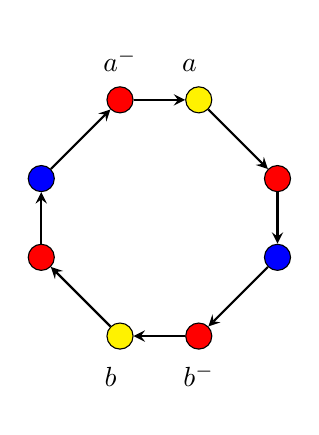
\begin{tikzpicture}[nodes={draw,circle,fill=black},arr/.style={thick,>=stealth,->}]

      \node[fill=red] (1) at (2,-1) {};
      \node[draw=none,fill=none] () at (2,-0.5) {$a^-$};
      \node[fill=yellow] (2) at (3,-1) {};
      \node[draw=none,fill=none] () at (3,-0.5) {$a^{\phantom{-}}$};
      \node[fill=red] (3) at (4,-2) {};
      \node[fill=blue] (4) at (4,-3) {};
      \node[fill=red] (5) at (3,-4) {};
      \node[draw=none,fill=none] () at (3,-4.5) {$b^-$};
      \node[fill=yellow] (6) at (2,-4) {};
      \node[draw=none,fill=none] () at (2,-4.5) {$b^{\phantom{-}}$};
      \node[fill=red] (7) at (1,-3) {};
      \node[fill=blue] (8) at (1,-2) {};

      \draw[arr] (1) -- (2);
      \draw[arr] (2) -- (3);
      \draw[arr] (3) -- (4);
      \draw[arr] (4) -- (5);
      \draw[arr] (5) -- (6);
      \draw[arr] (6) -- (7);
      \draw[arr] (7) -- (8);
      \draw[arr] (8) -- (1);

    \end{tikzpicture}%
    \qquad\qquad %
    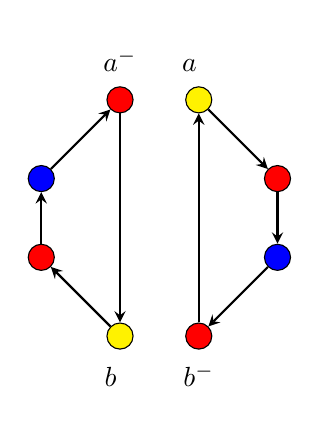
\begin{tikzpicture}[nodes={draw,circle},arr/.style={thick,>=stealth,->}]

      \node[fill=red] (1) at (2,-1) {};
      \node[draw=none,fill=none] () at (2,-0.5) {$a^-$};
      \node[fill=yellow] (2) at (3,-1) {};
      \node[draw=none,fill=none] () at (3,-0.5) {$a^{\phantom{-}}$};
      \node[fill=red] (3) at (4,-2) {};
      \node[fill=blue] (4) at (4,-3) {};
      \node[fill=red] (5) at (3,-4) {};
      \node[draw=none,fill=none] () at (3,-4.5) {$b^-$};
      \node[fill=yellow] (6) at (2,-4) {};
      \node[draw=none,fill=none] () at (2,-4.5) {$b^{\phantom{-}}$};
      \node[fill=red] (7) at (1,-3) {};
      \node[fill=blue] (8) at (1,-2) {};

      \draw[arr] (5) -- (2);
      \draw[arr] (2) -- (3);
      \draw[arr] (3) -- (4);
      \draw[arr] (4) -- (5);
      \draw[arr] (1) -- (6);
      \draw[arr] (6) -- (7);
      \draw[arr] (7) -- (8);
      \draw[arr] (8) -- (1);

    \end{tikzpicture}
    
    \end{center}
    
    \caption{Esempio delle strutture $A$ (sulla sinistra) e $B$ (sulla destra), per $\ell=8$.}
    \label{fig:grafi}
  \end{figure}

\end{proof}



\begin{teorema}
  $\ESOmon \neq \coESOmon$.
\end{teorema}

\begin{proof}
  Segue immediatamente dai Lemmi~\ref{lemma:connected-coESOmon} e \ref{lemma:connected-not-ESOmon}.
\end{proof}




\section{\texorpdfstring{$\NP$}{NP}-completezza di \texorpdfstring{$\SAT$}{SAT}}

Il Teorema~\ref{thm:np-eso} consente di dimostrare in modo particolarmente semplice l'$\NP$-com\-ple\-tez\-za del problema di soddisfacibilità booleana di formule proposizionali, denominato comunemente ``$\SAT$''.

\begin{teorema}
  $\SAT$ è $\NP$-completo.
\end{teorema}

\begin{proof}
  $\SAT$ appartiene a $\NP$, perché un certificato di soddisfacibilità di una formula è dato dal valore da assegnare alle variabili per fare in modo che la formula risulti vera.
  
  Dobbiamo dimostrare che un qualsiasi problema $\mathcal{A}\in\NP$ si riduce polinomialmente a $\SAT$.
  Supponiamo che $\mathcal{A}$ sia un insieme di strutture nel linguaggio $L=\{R_1,\dots,R_t\}$, dove $R_1,\dots,R_t$ sono relazioni di arietà $b_1,\dots,b_t$, rispettivamente.
  Per il Teorema~\ref{thm:np-eso} esiste una formula $\gamma$ della forma
  \[ \gamma :\equiv \exists\, S_1,\dots,S_r \, \forall \underbrace{x_1,\dots,x_n}_{\text{prim'ordine}} \, \underbrace{\varphi(x_1,\dots,x_k)}_{\text{senza quantificatori}} \]
  tale che $\mathcal{A}$ sia dato dai modelli di $\gamma$.
  
  Sia $A$ una $L$-struttura, e sia $n=|A|$. Abbiamo che $A$ appartiene a $\mathcal{A}$ se e solo se soddisfa la formula $\gamma$, ovvero se e solo se esistono delle relazioni $S_1^A\subseteq n^{a_1}, \dots, S_r^A\subseteq n^{a_r}$ tali che sia soddisfatta $\forall x_1,\dots,x_n \,\varphi(x_1,\dots,x_k)$.
  Questo è equivalente a trovare un'assegnazione che renda vera la formula proposizionale
  \[ \psi :\equiv \bigwedge_{0\leq c_1,\dots,c_k < n} \varphi(c_1,\dots,c_k) \]
  nelle varabili booleane $S_i(\vec{y})$ ed $R_j(\vec{z})$, al variare di $i\in \{1,\ldots,r\}$, $j\in\{1,\dots,t\}$, $\vec{y}\in n^{a_i}$, $\vec{z}\in n^{b_j}$.
  Sostituiamo a ciascuna variabile del tipo $R_j(\vec{z})$ il valore vero o falso, a seconda che valga o meno $A \models R_i(\vec{z})$; chiamiamo $\tilde\psi$ la formula così ottenuta, che dipende ora solamente dalle variabili $S_i(\vec{y})$ al variare di $i$ e di $\vec{y}\in n^{a_i}$.
  In conclusione, $A$ appartiene a $\mathcal{A}$ se e solo se esiste un'assegnazione delle variabili $S_i(\vec{y})$ che rende vera la $\psi$. Il numero di tali variabili è $n^{a_1}+\ldots+n^{a_r}$, che è un polinomio in $n$.
  Abbiamo quindi mostrato una riduzione polinomiale di $\mathcal{A}$ a $\SAT$.
\end{proof}
